\clearpage
\section{Analysis and results}
\label{sec:analysis}
In this section will elaborate the numerical analysis of the
data obtained in the measurements. We start with general remarks on the 
treatment of statistical errors applied. The next part covers the calibration 
of the histograms obtained with the two scintillators, using the known 
peaks of the two samples. The main part of the analysis consists of the 
examination of energy calibration and the comparison between theoretical 
prediction for differential and total cross sections with the experimental 
data. 

\subsection{Techniques used for the evaluation}
\label{sub:techique}
All calculations are done with scripts written in 
the \textit{python} programming language~\cite{python}, relaying in several 
packages:
\begin{itemize}
    \item
        \textit{matplotlib}~\cite{Hunter2007} for plotting,
    \item
        \textit{scipy}~\cite{scipy} for fitting, and 
    \item
        \textit{uncertainties}~\cite{uc} for error propagation.
\end{itemize}
The latter applies Gaussian error propagation for correlated and uncorrelated variables. 
We will thus not explicitly write down the formulas for the error propagation 
for each quantity calculated but instead state the numerical result only. 
We will, however make a quick remark on the use of covariance matrices in 
error propagation: Contrary to measured data, which in our case is usually 
expected to be uncorrelated, all fitted data yields variables that in general correlate. 
The propagation is then done as follows:
Let's assume we have random
variables $x_0,...,x_N$ which are correlated through the $N\times N$ Matrix $cov(x_i,x_j)$.
For a scalar function $f(x_0,...,x_N) \rightarrow \mathbb{R}$, the variance is estimated (linearly) by:
\begin{equation}
Var[f] = \sigma^2 = \sum_{i,j} \frac{\partial f}{\partial x_i} \frac{\partial f}{\partial x_j} cov(x_i,x_j) \,.
\end{equation} 
If instead, $\mathbf{f}$ is a vector field in $m$ dimensions, namely 
$\mathbf{f}(x_0,...,x_N) \rightarrow \mathbb{R}^m$, then the components of $\mathbf{f}$ 
are further correlated. We can write down the relation between the covariance matrices $V$ and $U$ of 
$\mathbf{x}$ and $\mathbf{f}$, respectively, in matrix relations:
\begin{equation}
    U = A V A^T
\end{equation}
where $A$ is the matrix defined by 
\begin{equation}
    A_{ij} = \left[ \frac{\partial f_i}{\partial x_j}\right]_{\mathbf{x} = \mu}
\end{equation}
with expectation value $E[\mathbf{x}] = \mu$.~\cite{cowan1998statistical}

\subsection{Calibration of PVC scintillator}
\label{sub:calibration}
The purpose of this section is to calibrate the channels obtained by the MCA to
known energies. In order to compare between measurements, we transform the measured 
histograms to rates by dividing each count by the total time measured. 
\begin{equation}
    \text{rate: } n(channel)  = 	\frac{N(channel)}{T}
    \label{eq:rate}
\end{equation}

Then we subtract for each channel the background rate, which
was calculated analogously 
\begin{equation}
    n_\mathrm{cleansed} = n - n_\mathrm{background}.
    \label{eq:rate2}
\end{equation}
This procedure will be used in all calculations below without explicit restating. 
The error propagation is done according to section~\ref{sub:techique}.
The Compton edge is approximated in first order by an Heaviside step function,
convoluted\footnote{ 
    A convolution is defined by
\begin{equation}
    a \star b   \stackrel{\mathrm{def}}{=}\ \int_{-\infty}^\infty a(\tau)\, b(t - \tau)\, d\tau 	
    \label{eq:conv}
\end{equation}

} with an Gaussian to take into account the smearing
effects if the detector:
\begin{equation}
    n(E)  \approx A\cdot \Theta(E_0 - E) \star  	
    \left[  \frac{1}{\sqrt{2\pi\sigma^2}} \exp \left( 
        \frac{-(E-E_0)^2}{2\sigma^2}\right)
        \right]  =\frac{A}{2^{3/2}\sigma} 
    \mathrm{erfc}(E - E_0) 
    \label{eq:errorfunc}
\end{equation}
With the amplitude A and the inverse error function
\begin{equation}
    \mathrm{erfc}(x) = 1 - \mathrm{erf}(x) , \quad
    \operatorname{erf}(x) = 
    \frac{2}{\sqrt\pi}\int_0^x e^{-t^2}\,\mathrm dt. 
    \label{eq:erfc}
\end{equation}
We will use this approximation for the fit of all Compton 
edges. In the case of more than one Compton edges, we just
sum them up. For all fits an additional fitting parameter 'offset'
is used for taking into account probable noise or background
effects, which could not be eliminated by subtracting the 
measured background rate. For the photon and escape peaks we use 
a simple Gaussian, as it appears in equation \eqref{eq:errorfunc}.
The fits are done using least squares minimization (see 
\cite{scipy} for a reference of the fitting algorithm), where 
we include absolute the errors of the respective y-axis as 
weights. Please note
that we do not include the $\chi^2/\mathrm{dof}$ in all of the fits,
as we think this is not of particular interest and would lead
to confusing figures showing too much information. Our errors
of the rates are mostly estimated using $\sqrt(N)/T$, and hence
the $\chi^2/\mathrm{dof}$ are dependent 
on the measurement time, which we already know and
is given in the figures. The uncertainty of the fits and their
respective convergence is reflected in the errors of the 
results. 
%When necessary, we included the $\chi^2/\mathrm{dof}$,
%for instance in the linear fit of the calibration.\\

First we find for $^{22}$Na two Compton edges (341 keV and
1064 keV~\cite{nist}). The result is
channel $108 \pm 2$ and $414 \pm 4$ with a correlation of about 50\%, see
figure~\ref{fig:calib_ps_na}.

\begin{figure}[htpb]
    \centering
    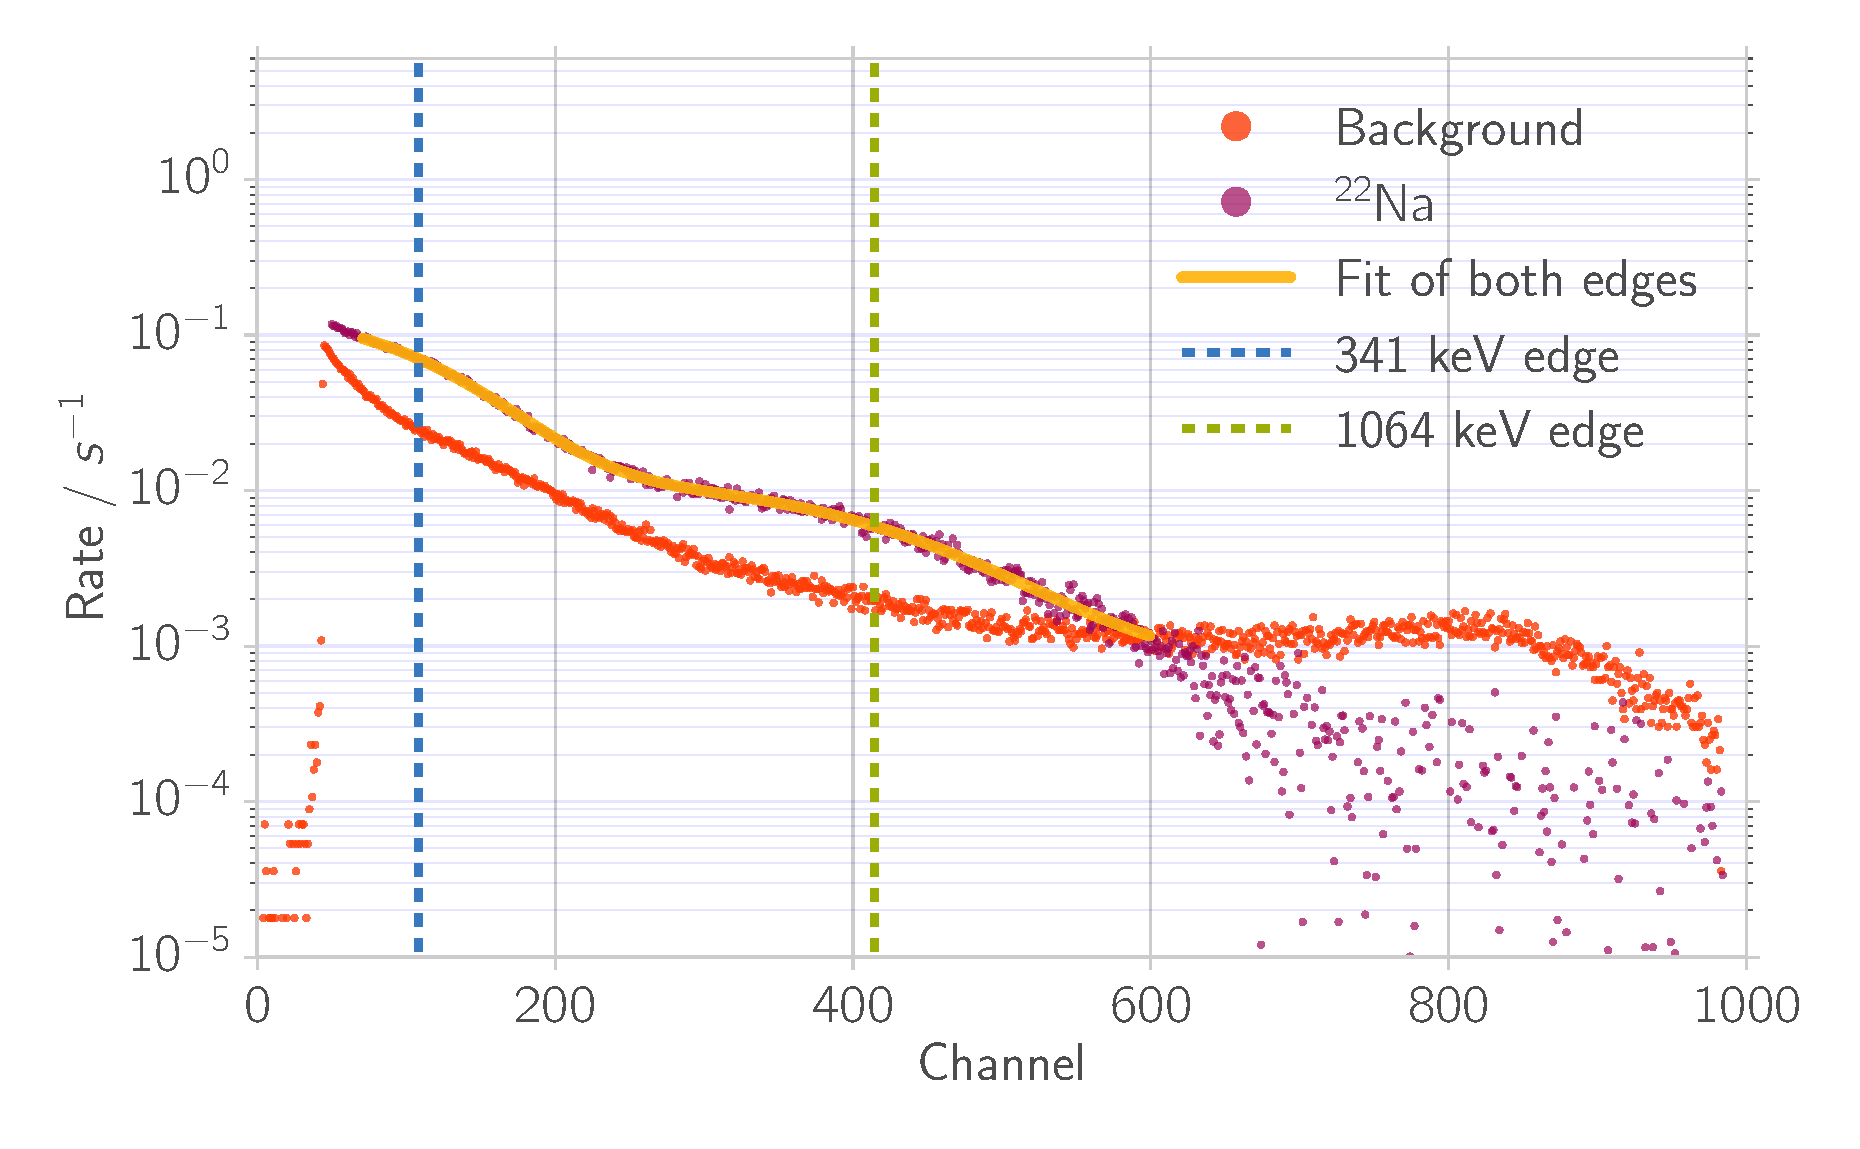
\includegraphics[width=0.9\linewidth]{./analysis/figures/calib_ps_na}
    \caption{Calibration of the PVC scintillator with
        $^{22}$Na sample (measurement time
    16.5 h) with refined background (measurement time 15.6h).
    Notice that the rate is 
    only fitted for the section in which the background is
    smaller than the sample. We
    subtracted the background rate at each channel
    for the sample in order not to fit the 
    behavior of the noise. The error of the two
    Compton edges is large (see text) coming
    from the fit and their high correlation coefficient. The 
dotted line refers to the displacement $E_0$ in \eqref{eq:errorfunc} which should resemble the position of the Compton
edge without convolution of a Gaussian, which was estimated
by the least squares fit.}
\label{fig:calib_ps_na}
\end{figure}
For $^{137}$Cs a Compton edge (477 keV~\cite{nist})
we found channel $178.9 \pm 0.3$ 
(notice the much smaller error compared to the $^{22}$Na sample), 
see figure~\ref{fig:calib_ps_cs} for the data and the fit.
\begin{figure}[htpb]
    \centering
    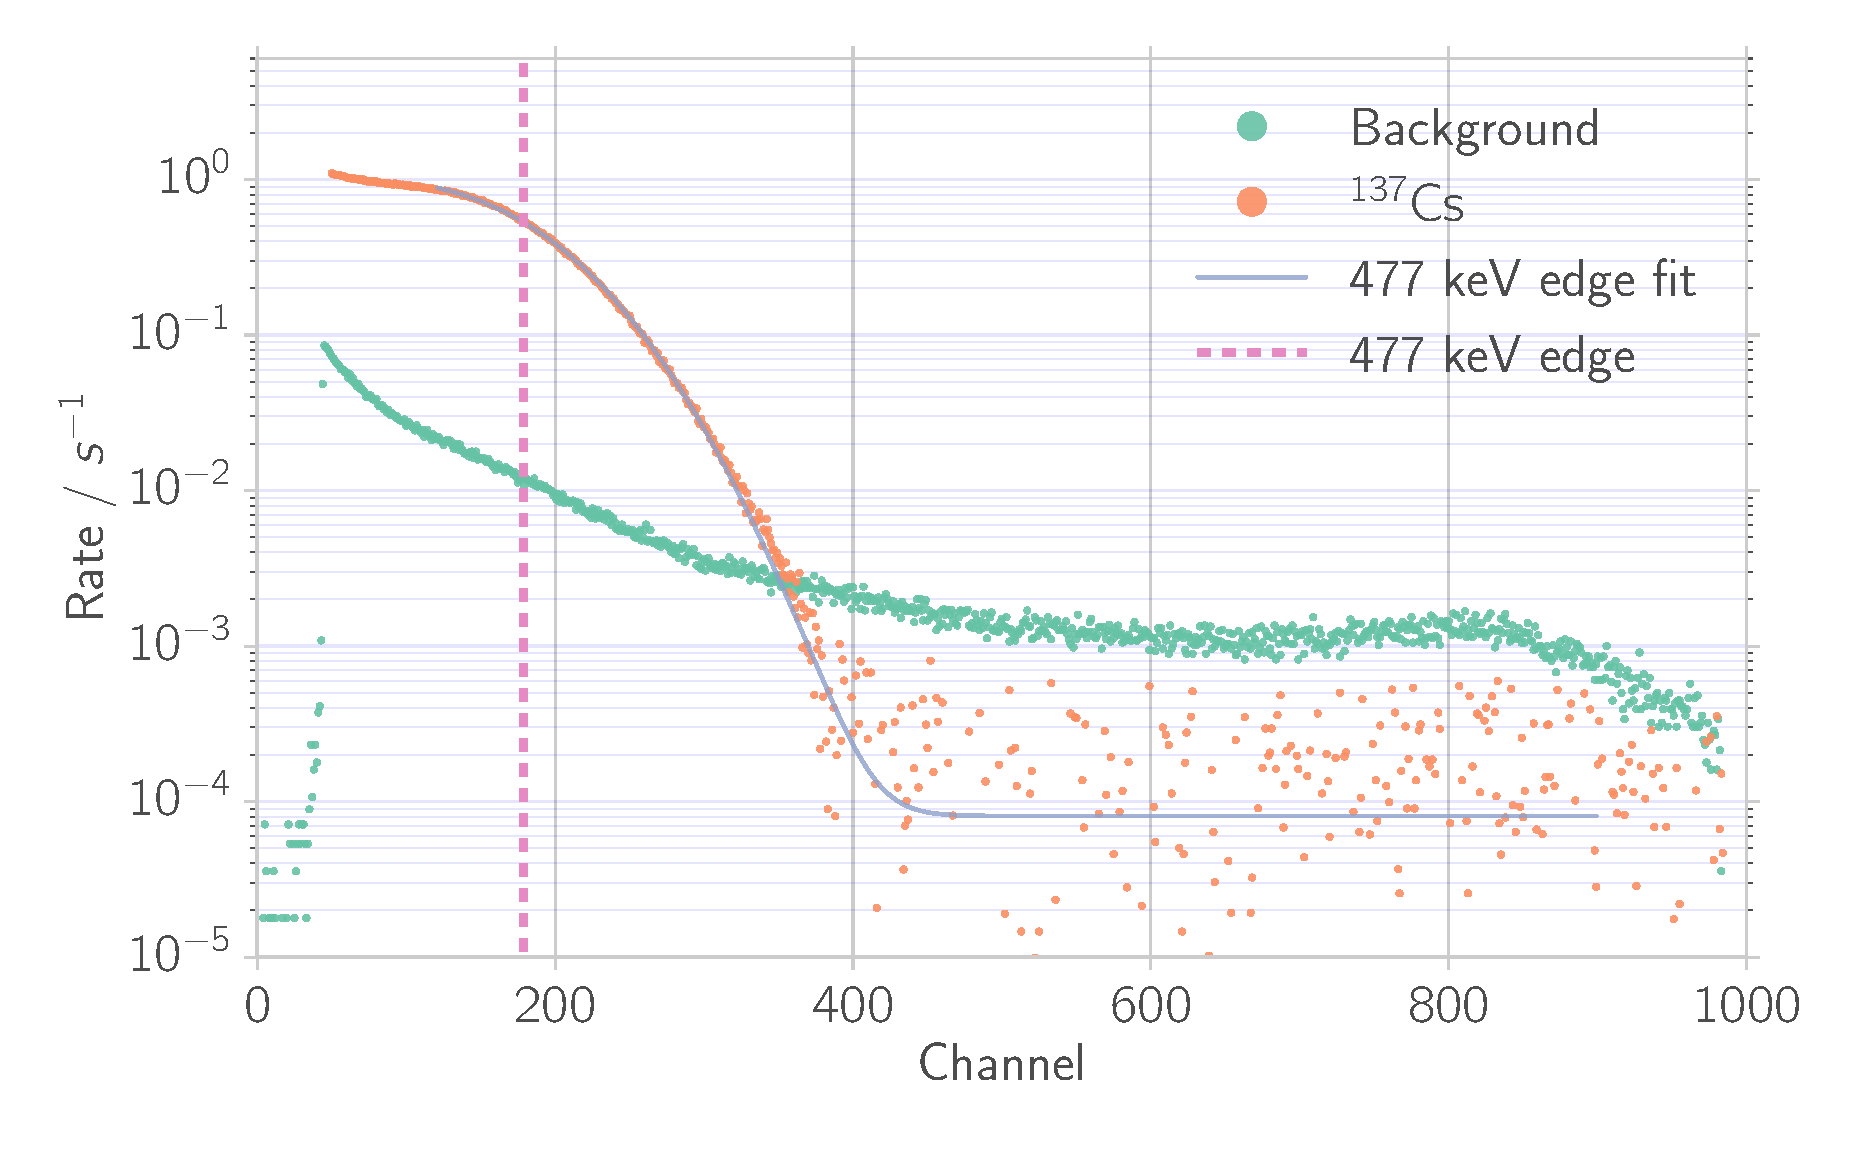
\includegraphics[width=0.9\linewidth]{./analysis/figures/calib_ps_cs}
    \caption{Calibration of the PVC scintillator with $^{137}$Cs sample. Measurement time
    6 h. We subtracted the background rate at each channel. }
\label{fig:calib_ps_cs}
\end{figure}

\begin{figure}[htpb]
    \centering
    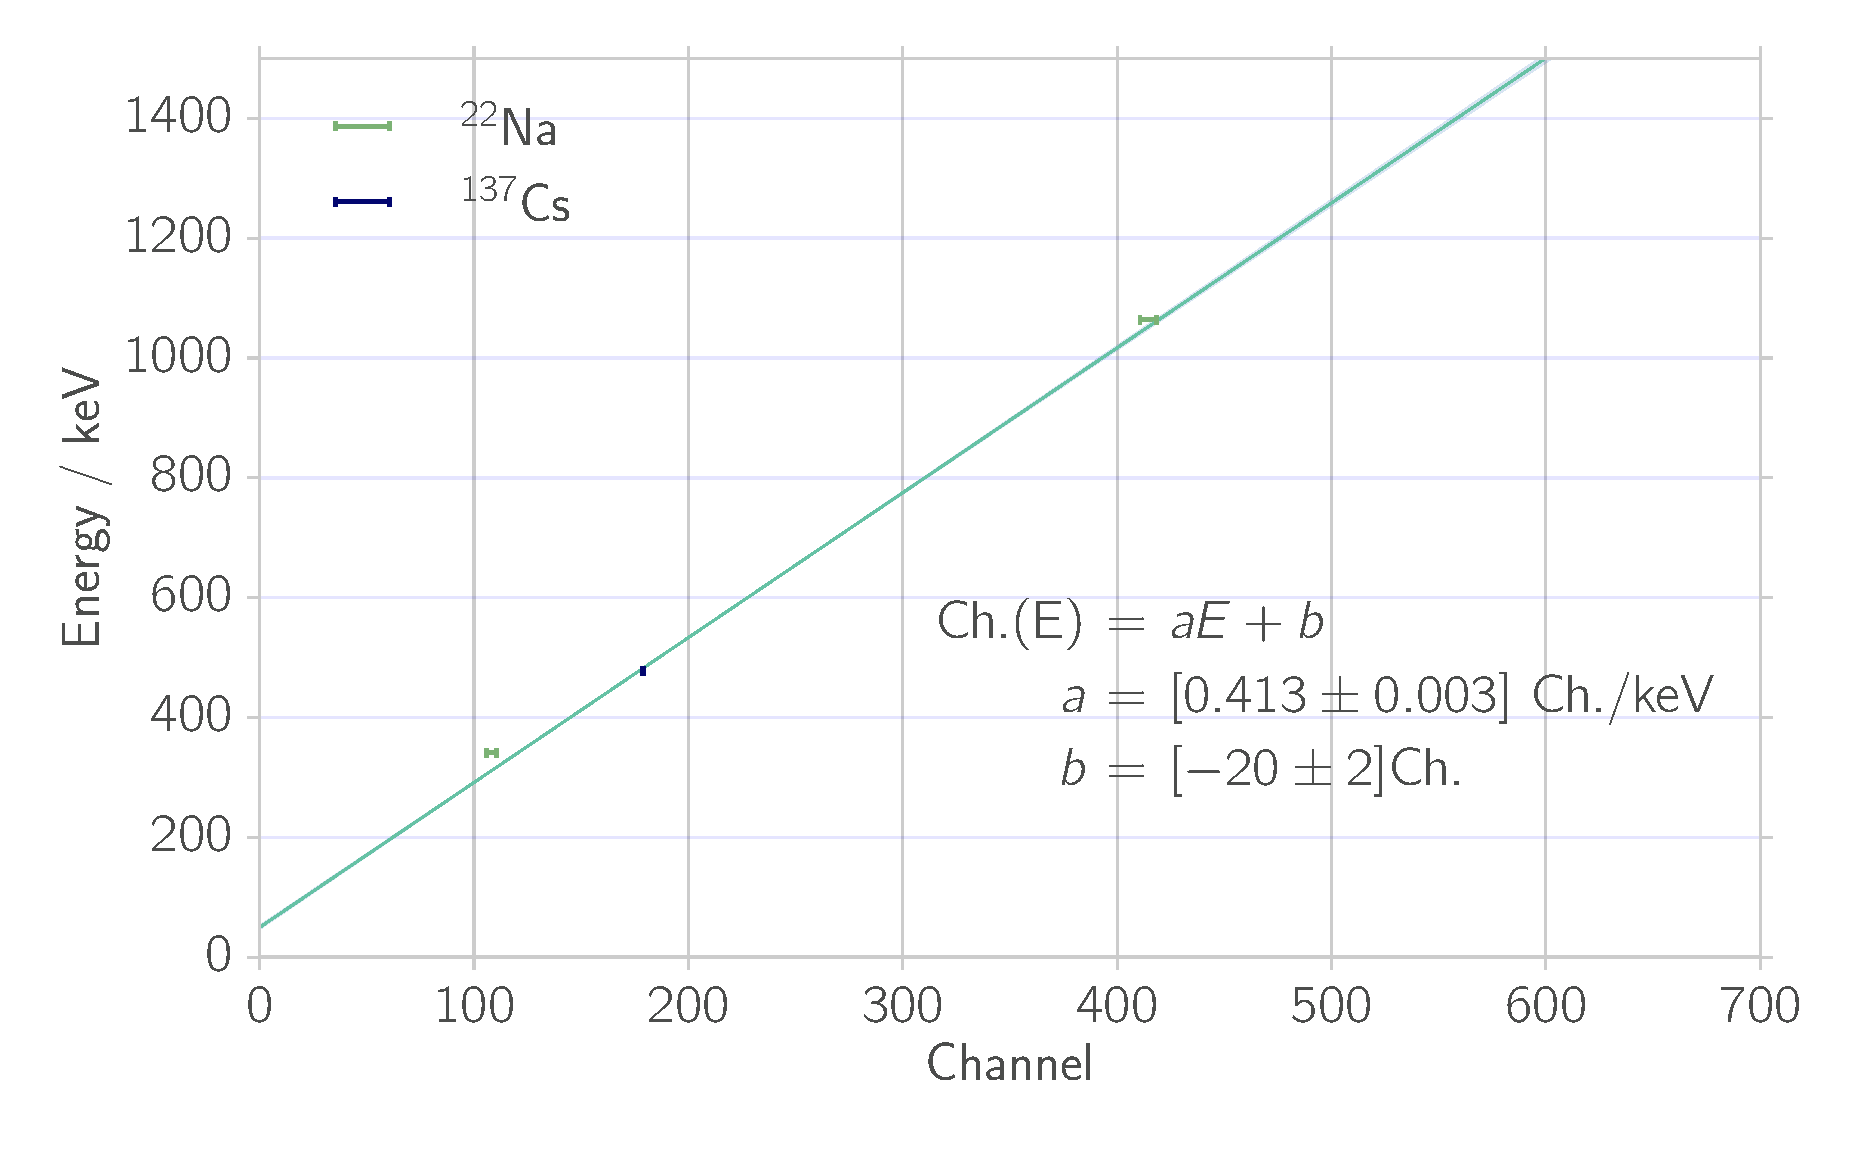
\includegraphics[width=0.9\linewidth]{./analysis/figures/calibration_ps_linear_fit}
    \caption{This is the result of the three Compton edges. We will use this calibration
    for all the following calculations. Note that statements about the error and linearity of the MCA 
    are not possible due to the low number of data points (which also the reason for
the $\chi^2/\mathrm{dof}$ to be $\infty$).}
\label{fig:calibration_ps_linear_fit}
\end{figure}
The final result of the linear calibration can be seen in
figure~\ref{fig:calibration_ps_linear_fit}.

\subsection{Calibration of NaI scintillator}

\label{sub:calibration_of_na_scintillator}
As in the last section we calculate a calibration, this time for the NaI scintillator. The
first figure~\ref{fig:histo_na_137cs} shows the spectrum of the $^{136}$Cs sample 
whereas the data for
$^{22}$Na can be seen in figure~\ref{fig:histo_na_22na} and figure~\ref{fig:histo_na_22na2}.
The results of the peak fits as well as literature values are displayed in the tables~\ref{tab:peaks_cs_ps}
and \ref{tab:peaks_na_ps} for each of the two samples. The literature values are fitted over peak positions, see 
figure~\ref{fig:calibration_na_linear_fit}, in order to yield a calibration. 
\begin{table}[htpb]
    \centering
    \caption{Peaks and fitting results of $^{137}$Cs~\cite{nist}.}
\label{tab:peaks_cs_ps}
    \begin{tabular}{lll}
        \rowcolor{LightCyan} Name &Energy & Channel \\ 
        Photo peak & 662 keV & $8049.41 \pm 0.03$\\ 
        Compton edge & 477 keV & $5720 \pm 4$\\  
        Escape peak & 183 keV & $2518 \pm 12$
    \end{tabular}
\end{table}

\begin{figure}[htpb]
    \centering
    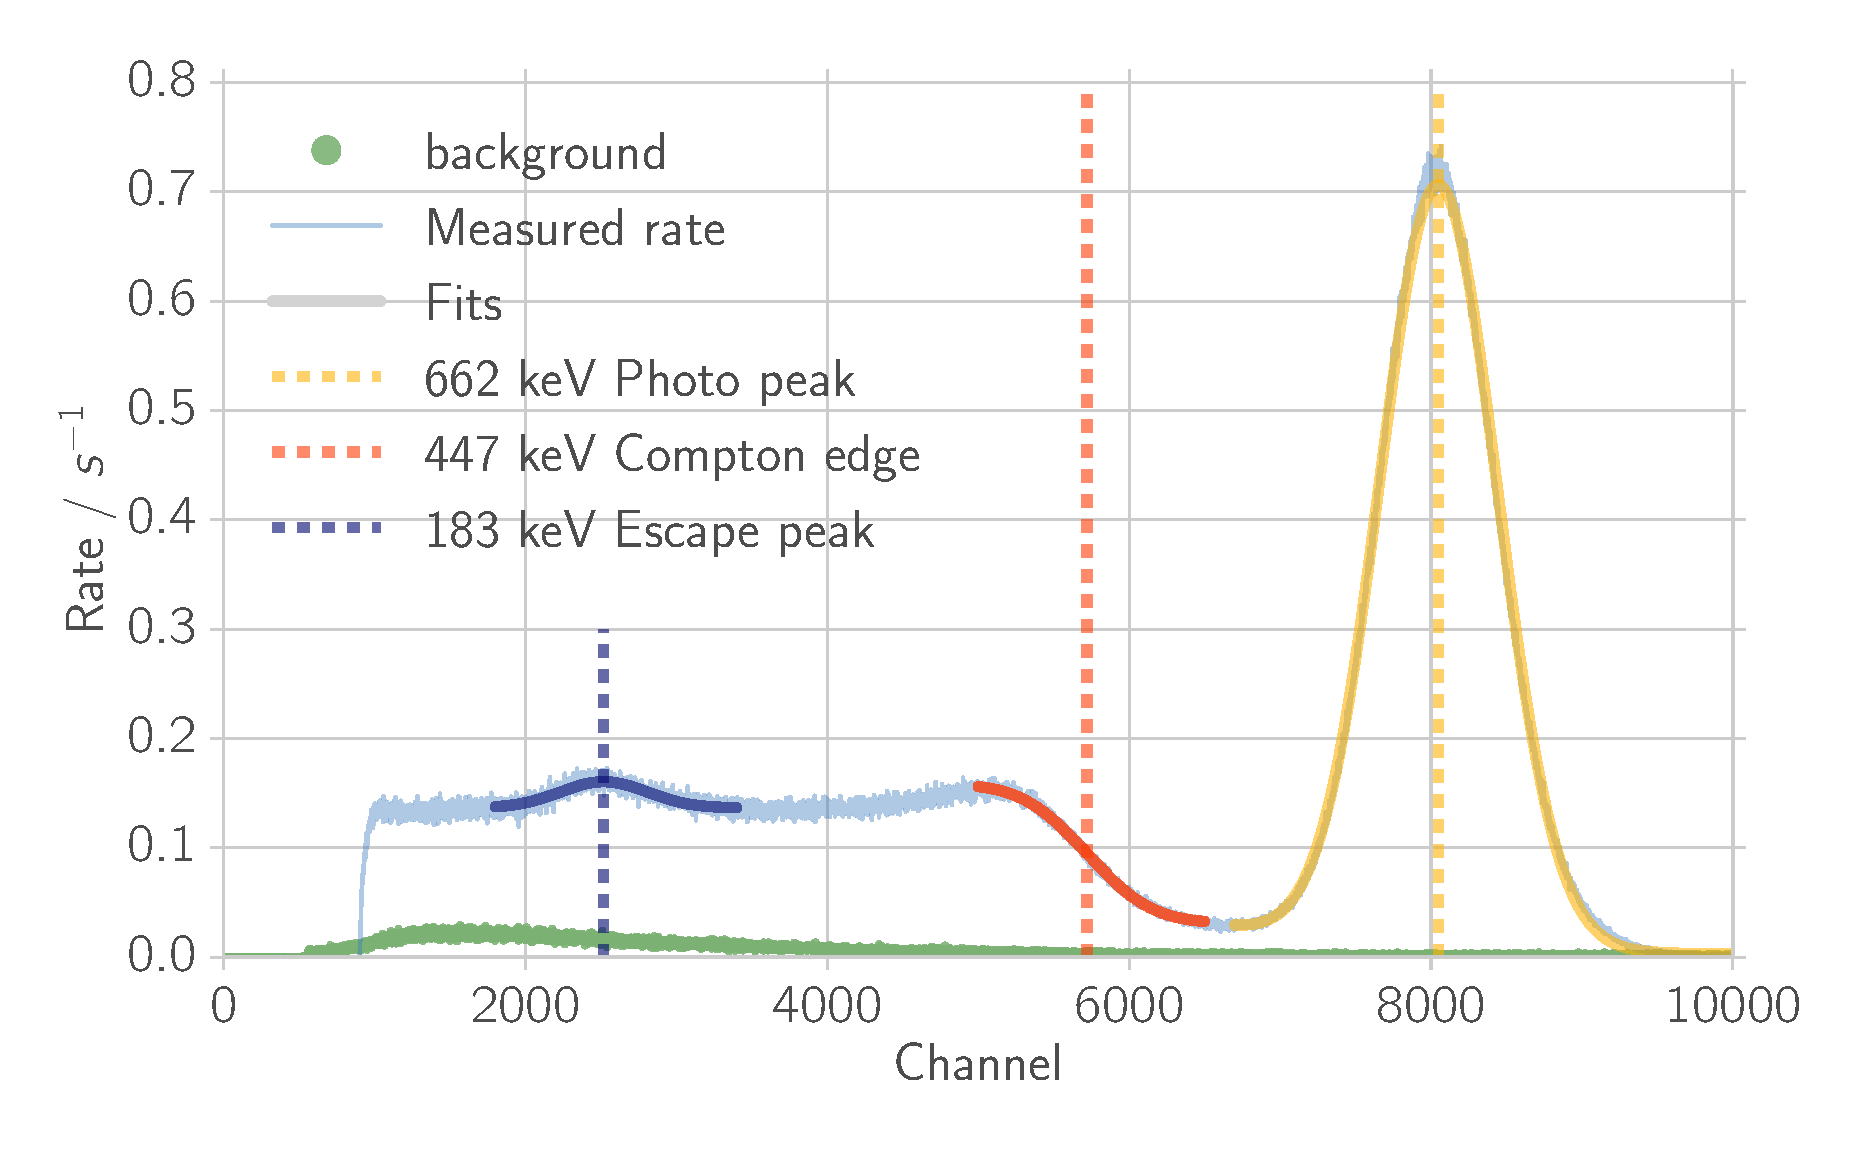
\includegraphics[width=0.9\linewidth]{./analysis/figures/histo_na_137cs}
    \caption{Calibration of the NaI scintillator using $^{137}$Cs sample (measurement
    time 2.7h) with refined background (measurement time 1h). }
\label{fig:histo_na_137cs}
\end{figure}

\begin{figure}[htpb]
    \centering
    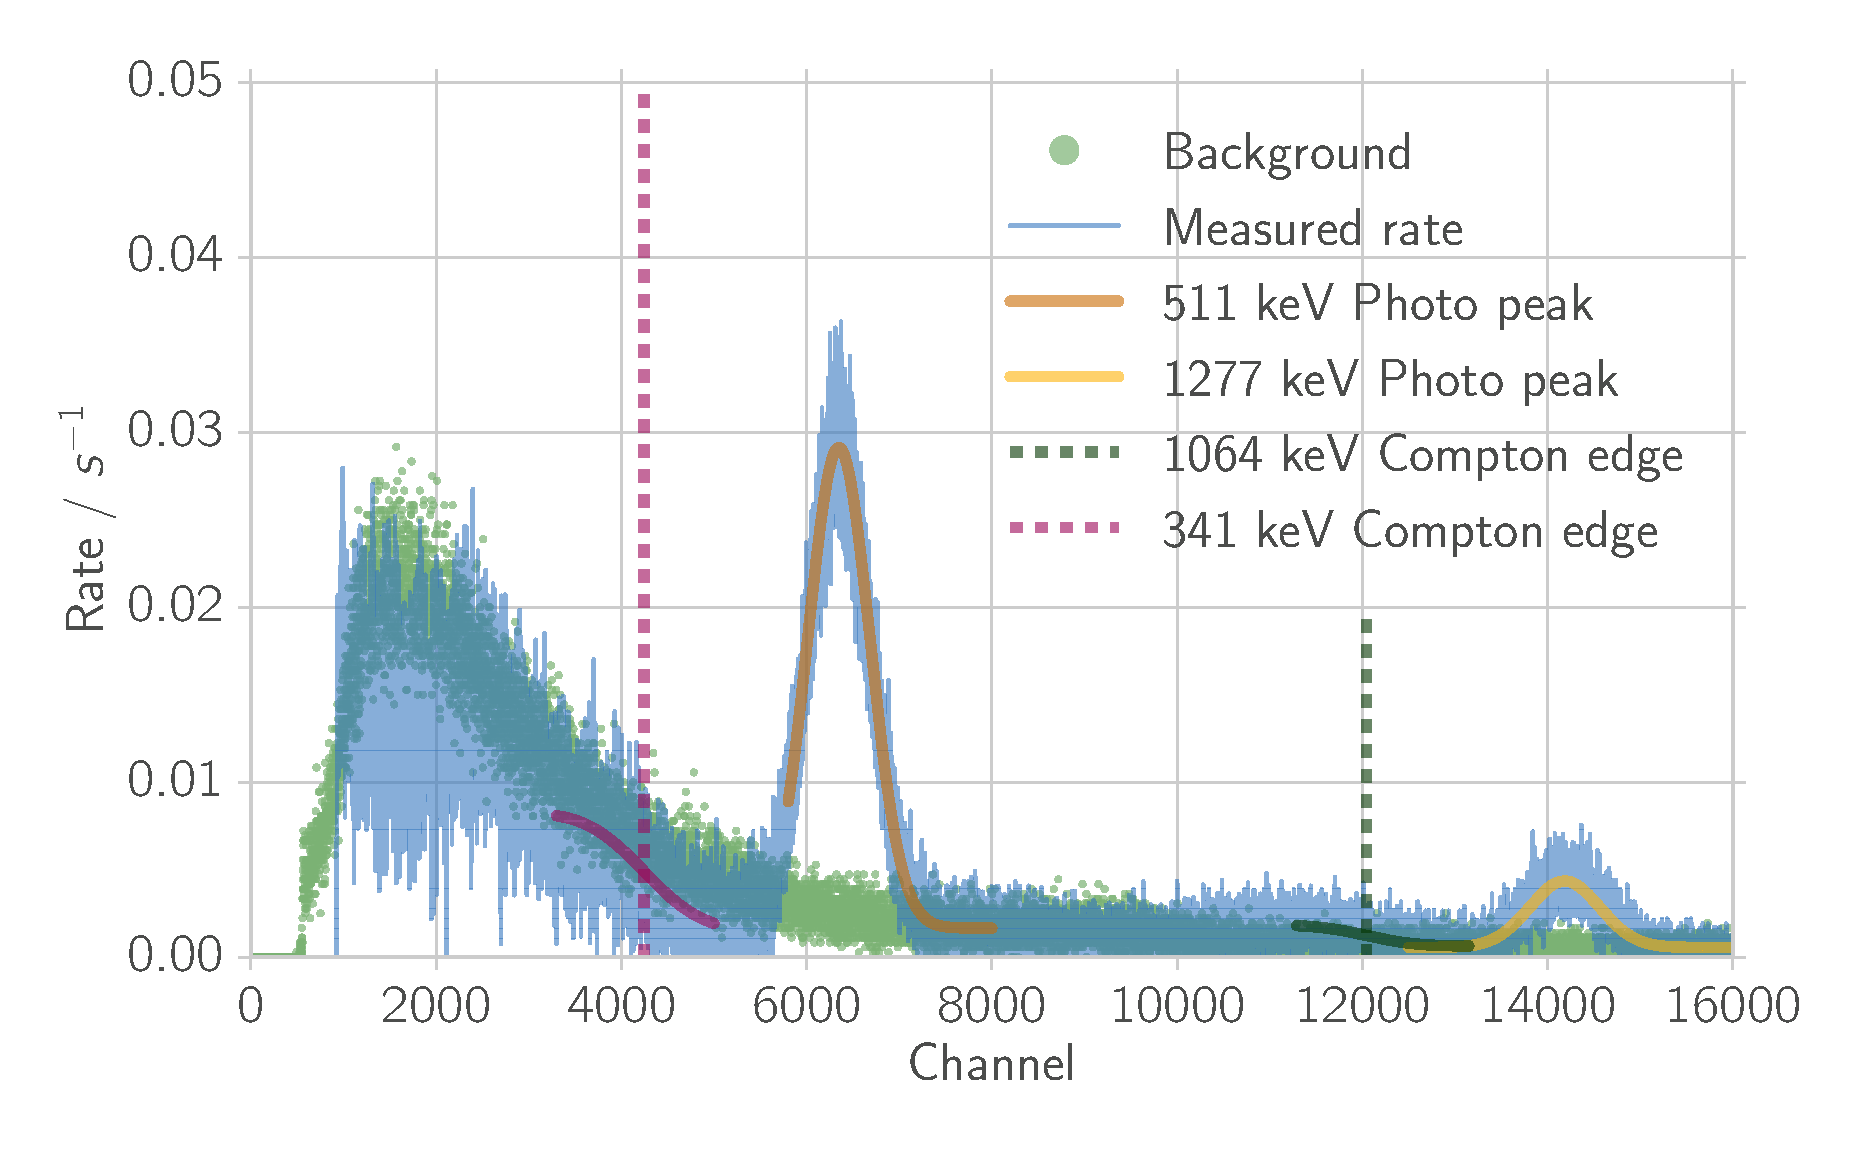
\includegraphics[width=0.9\linewidth]{./analysis/figures/histo_na_22na}
    \caption{Calibration of the NaI scintillator using $^{22}$Na sample (measurement
        time about 1h) with refined background (same as in figure~\ref{fig:histo_na_137cs},
        measurement time 1h). }
\label{fig:histo_na_22na}
\end{figure}

\begin{figure}[htpb]
    \centering
    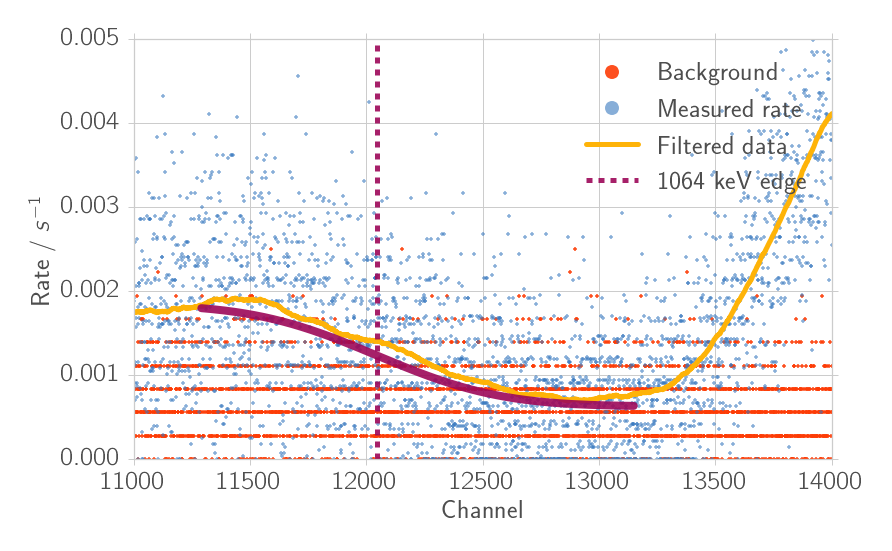
\includegraphics[width=0.9\linewidth]{./analysis/figures/histo_na_22na2}
    \caption{Enlargement of the critical area of the Compton edge of
    figure~\ref{fig:histo_na_22na}.     
    The red line is a Savitzky-Golay filter 
    with a width of 1001 points in the channel and a fourth
    degree polynomial applied to the data (see~\cite{scipy} for reference) in order
    to see the slope of the curve. The least-squares fit uses the real data, though.
}
\label{fig:histo_na_22na2}
\end{figure}

\begin{table}[htpb]
    \centering
    \caption{Peaks and fitting results of $^{22}$Na. As it is also visible in the figure
    of the leasts-squares fit~\ref{fig:calibration_na_linear_fit} the errors on the
    Compton edges are much higher than those of the Photo peaks. This is due to the high
    degree of uncertainty of the particular edge resulting from the fit. However, the 
    uncertainty of the linear fit is much less in the end.}
\label{tab:peaks_na_ps}
\begin{tabular}{lll}
    \rowcolor{LightCyan} Name &Energy & Channel \\ 
       1. Photo peak& 511 keV & $6348 \pm 3$ \\ 
       2. Photo peak& 1277 keV & $14190 \pm 30 $\\
       1. Compton edge& 341 keV& $4000 \pm 2000$\\
       2. Compton edge& 1064 keV & $12000 \pm 4000$
    \end{tabular}
\end{table}

\begin{figure}[htpb]
    \centering
    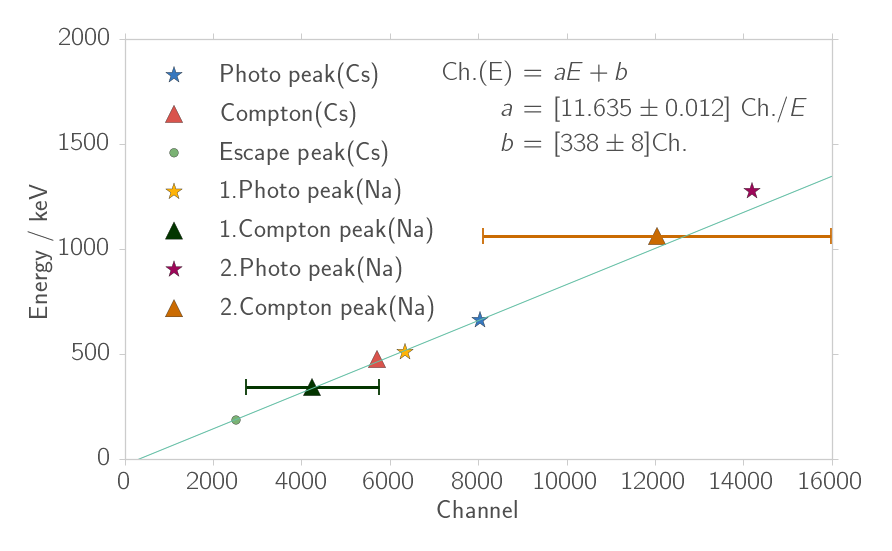
\includegraphics[width=0.9\linewidth]{./analysis/figures/calibration_na_linear_fit}
    \caption{All peaks measured by the NaI scintillator with the respective linear fit. The errors on 
        most of the peaks are too small to be shown, only the Compton peaks of $^{22}$Na show
        an exorbitant error. The second photo peak ($^{22}$Na sample) seems to be quite apart from
    the result of the other values; this might be due to a general systematic error. Our explanation is as following: 
    For Channels higher than a certain value, we experience the saturation of the MCA. This leads to a confusion about the
    real energy of the channel, since even higher energies might be placed into the same channel. Even though the error for the
    fit is low, the shift due to this effect causes a systematic shift. Therefore we excluded this peak, but this did not 
    change the slope of our linear fit, so we tend to neglect the effect of the systematic error in future calculations. }

\label{fig:calibration_na_linear_fit}
\end{figure}
\clearpage
\subsection{Energy conservation}
\label{sub:energy_conservation}
In this section we work out the dependence of the energy with respect to the scattered
angle. Figure~\ref{fig:coin_ps_background} shows the background (with
coincident setup but without sample) and random coincidences.
We subtract the background from our data before pursuing the analysis.
This will include evaluating a number of different measurements; we will
only show two example figures for each detector 
(figures~\ref{fig:coin_ps_90} and~\ref{fig:coin_ps_15} for the PVC scintillator and 
~\ref{fig:coin_na_90} and~\ref{fig:coin_na_30} for the NaI scintillator). The main
result is summarized in figure~\ref{fig:coin_na_90}. It shows the expectation values of
the energy, dependent on different scattering angles $\theta$.


\begin{figure}[htpb]
    \centering
    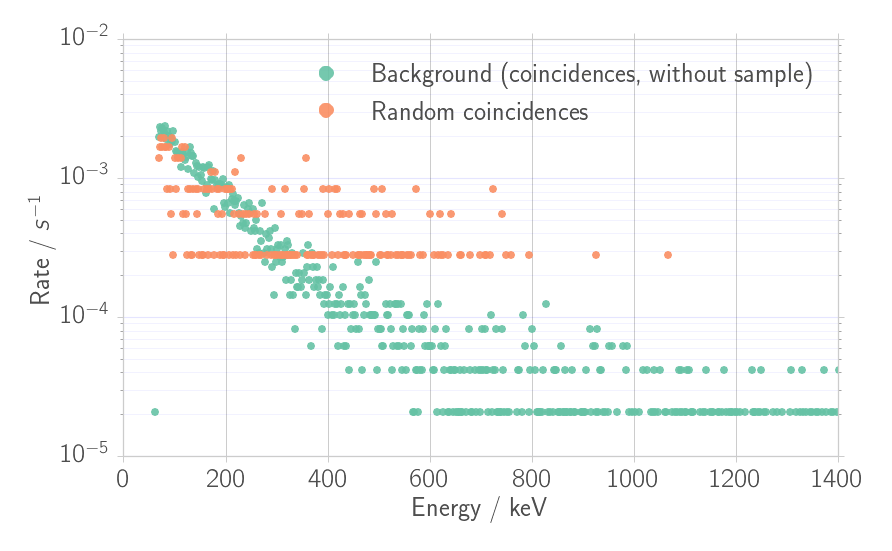
\includegraphics[width=0.9\linewidth]{./analysis/figures/coin_background_random}
    \caption{Background and random coincidences of the PVC scintillator. 
        The background is measured in coincident setup for 13.4h, the random coincidences are 
    measured with the $^{137}$Cs sample inserted (measurement time 1h).}
\label{fig:coin_ps_background}
\end{figure}

\begin{figure}[htpb]
    \centering
    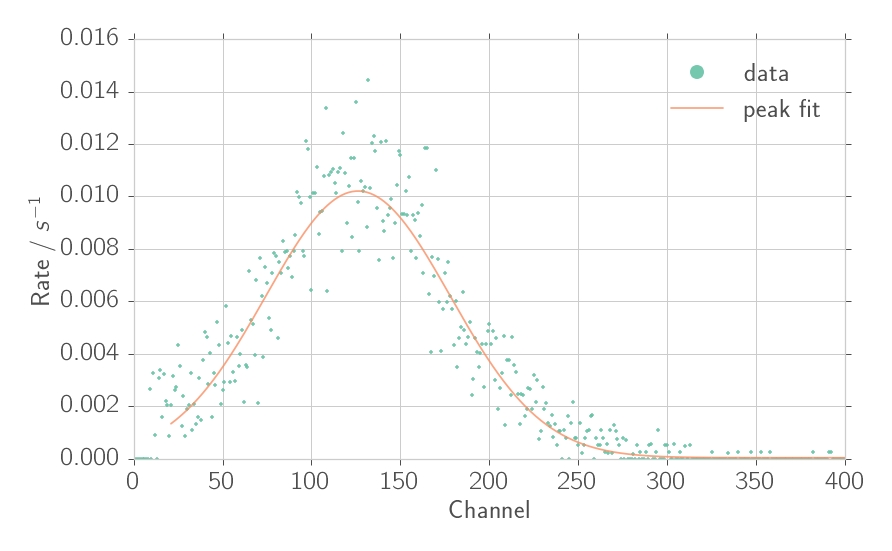
\includegraphics[width=0.9\linewidth]{./analysis/figures/coin_ps_90}
    \caption{\textbf{Energy of electrons:}
    Rate of coincident events of PVC scintillator at angle of $\theta = 90^\circ$ 
        (measurement time 1h). The distribution 
    was approximated with a Gaussian distribution. }
\label{fig:coin_ps_90}
\end{figure}

\begin{figure}[htpb]
    \centering
    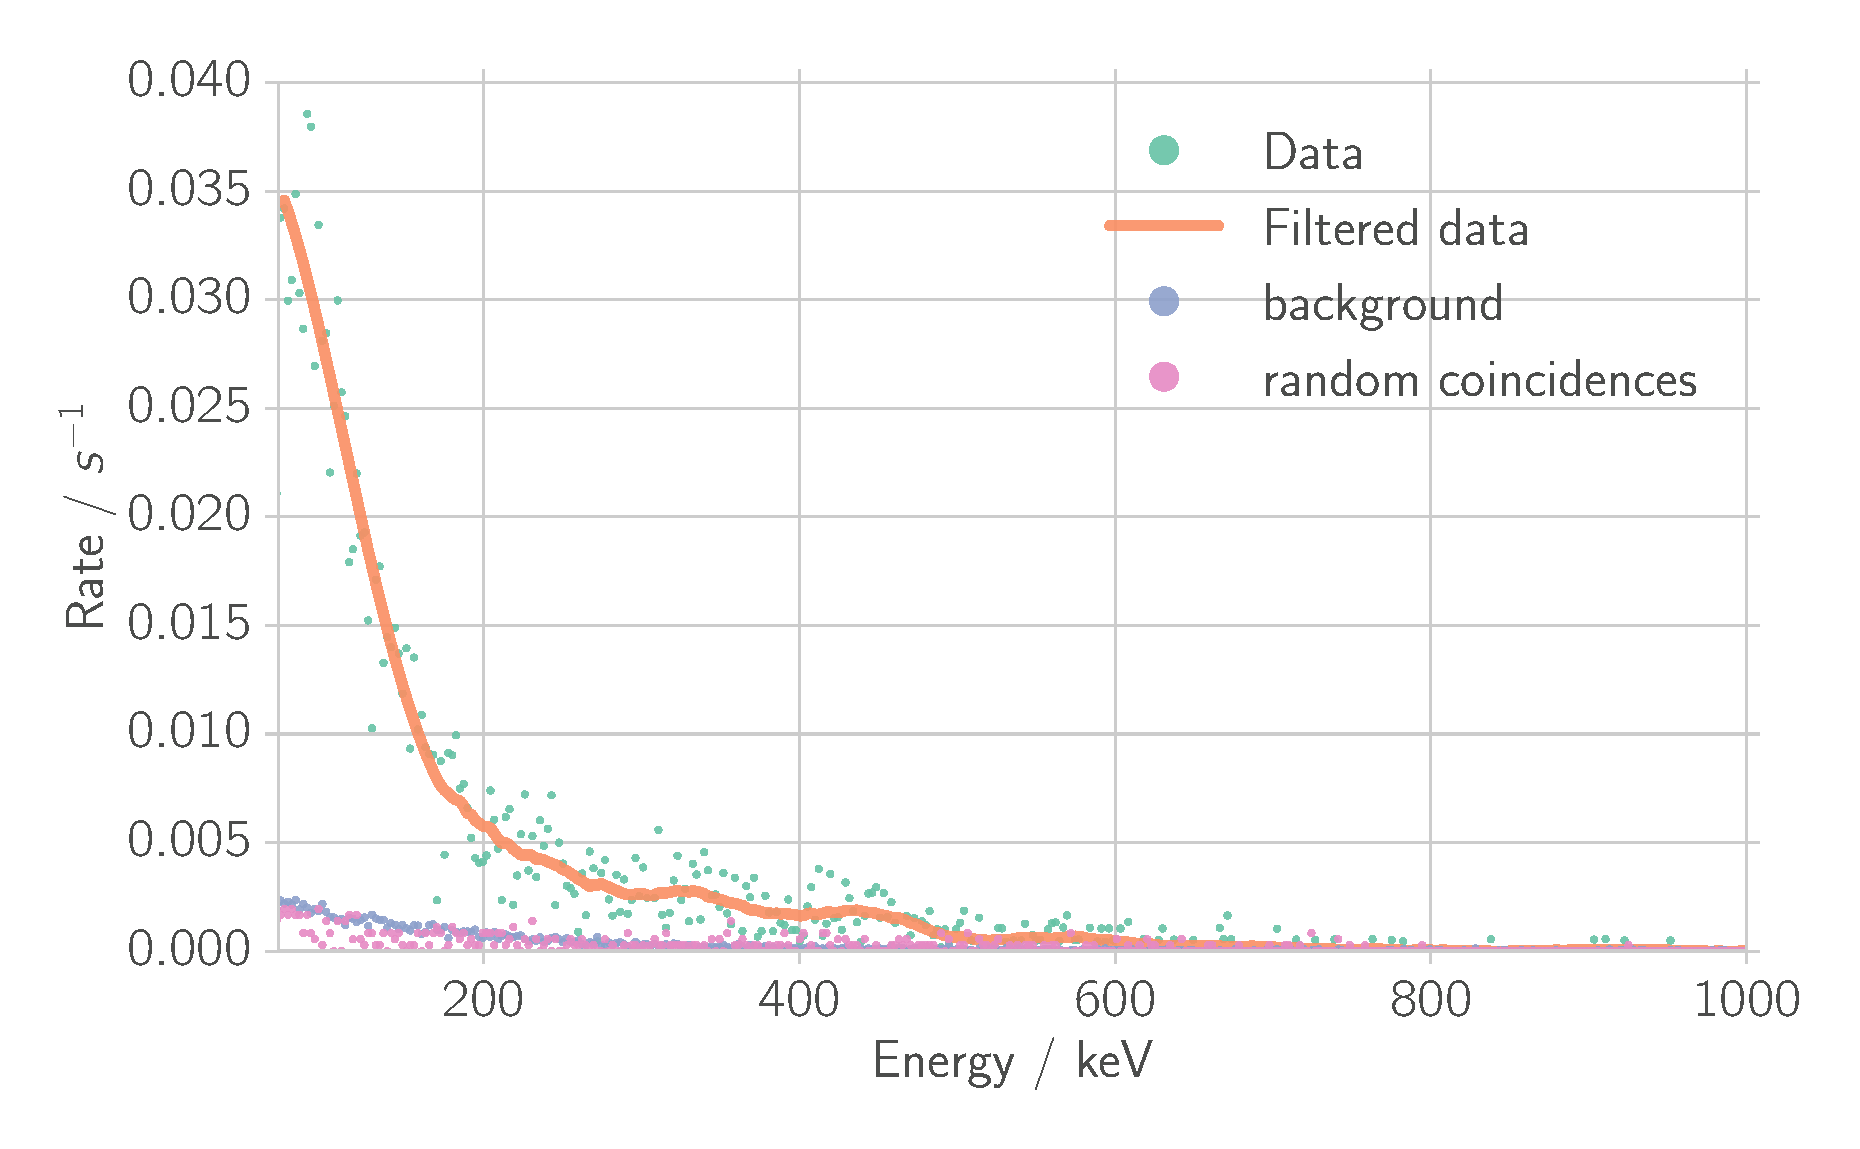
\includegraphics[width=0.9\linewidth]{./analysis/figures/coin_ps_15_filter_}
    \caption{\textbf{Energy of electrons:}
        Rate of coincident events of 
        PVC scintillator at angle of $\theta = 15^\circ$.
        In this figure we used, unlike at higher angles, applying the Savitzky-Golay filter
        with a width of 81 points and a fourth
        degree polynomial (see~\cite{scipy} for reference). This was done for 
        angles $\theta = 15^\circ$ up to $\theta = 60^\circ$.}
\label{fig:coin_ps_15}
\end{figure}

\begin{figure}[htpb]
    \centering
    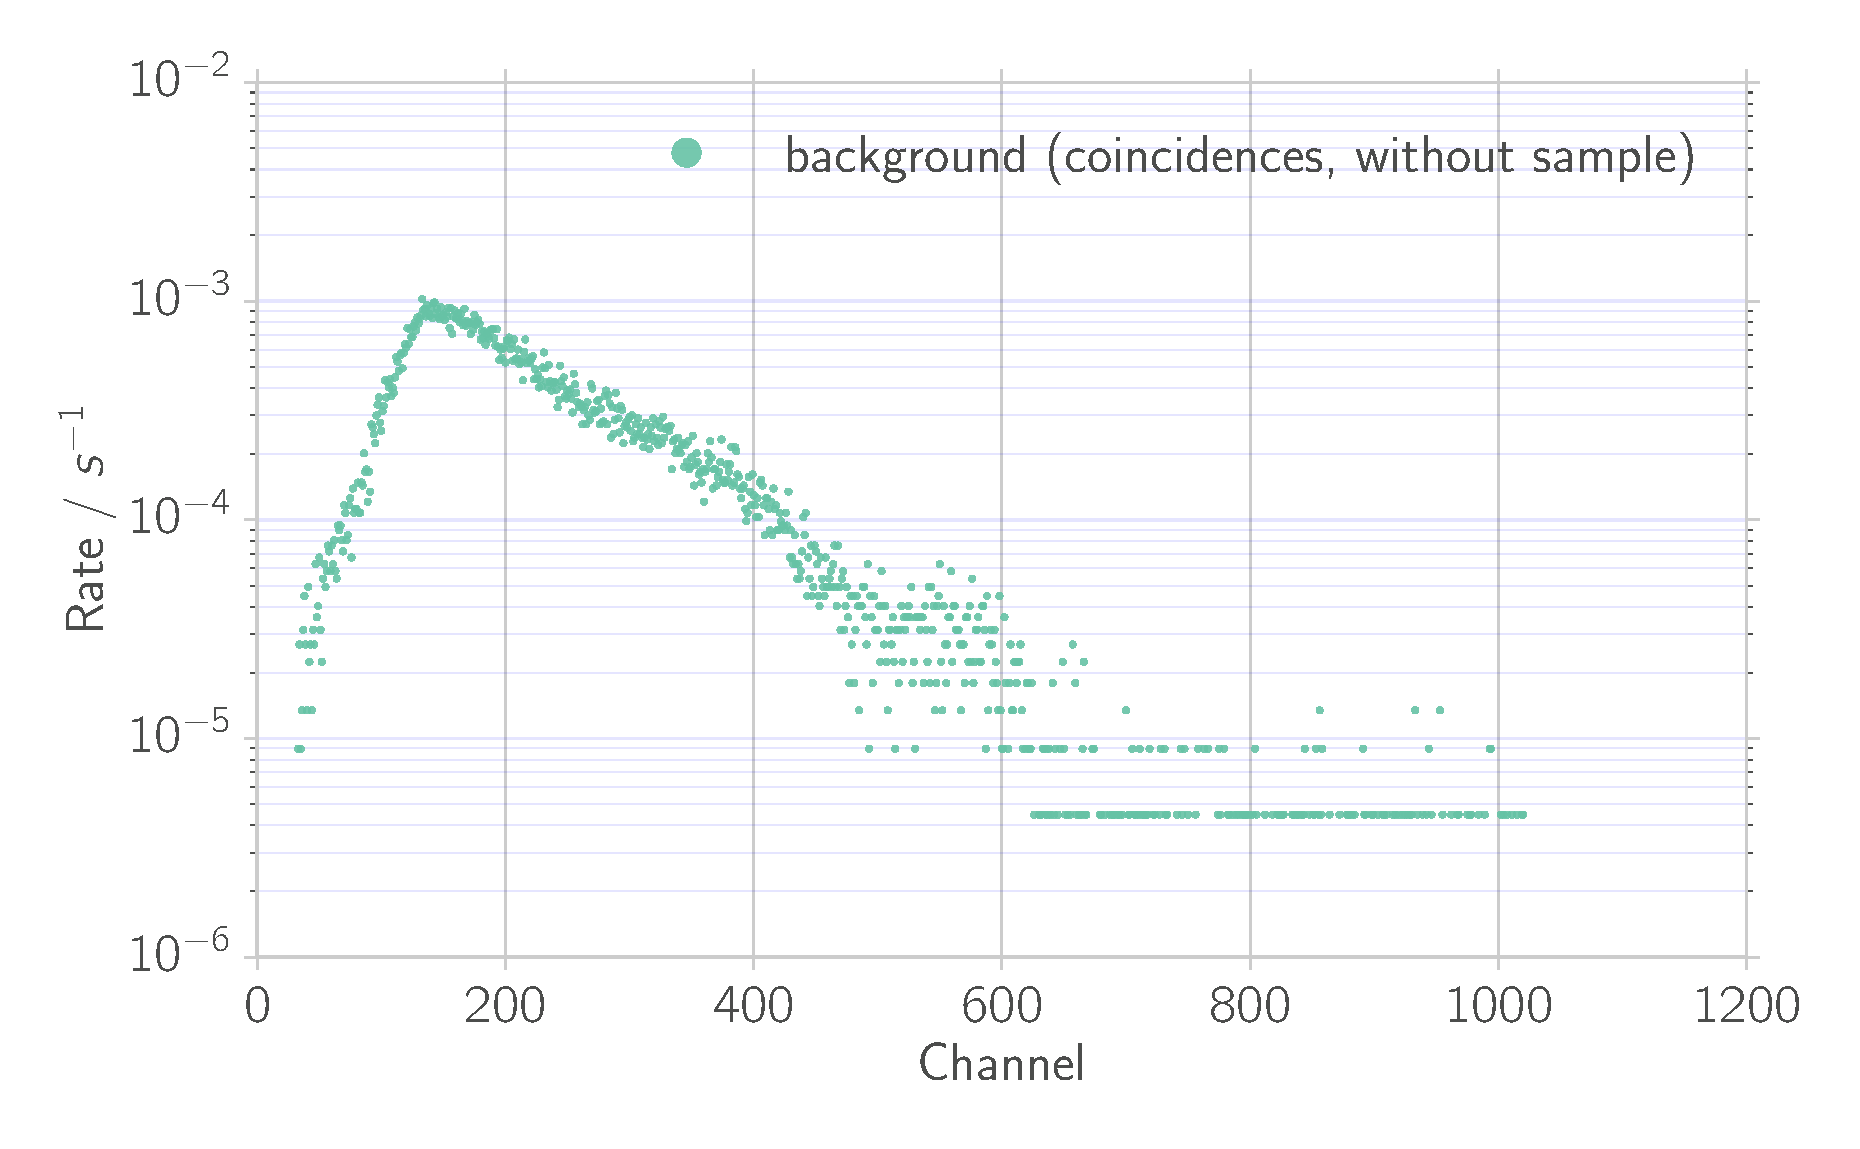
\includegraphics[width=0.9\linewidth]{./analysis/figures/coin_na_background}
    \caption{Background in coincident setup for the NaI scintillator, measured for 62h. Note that we receive the clear shape because of the long measurement. } \label{fig:coin_na_background}
\end{figure}

\begin{figure}[htpb]
    \centering
    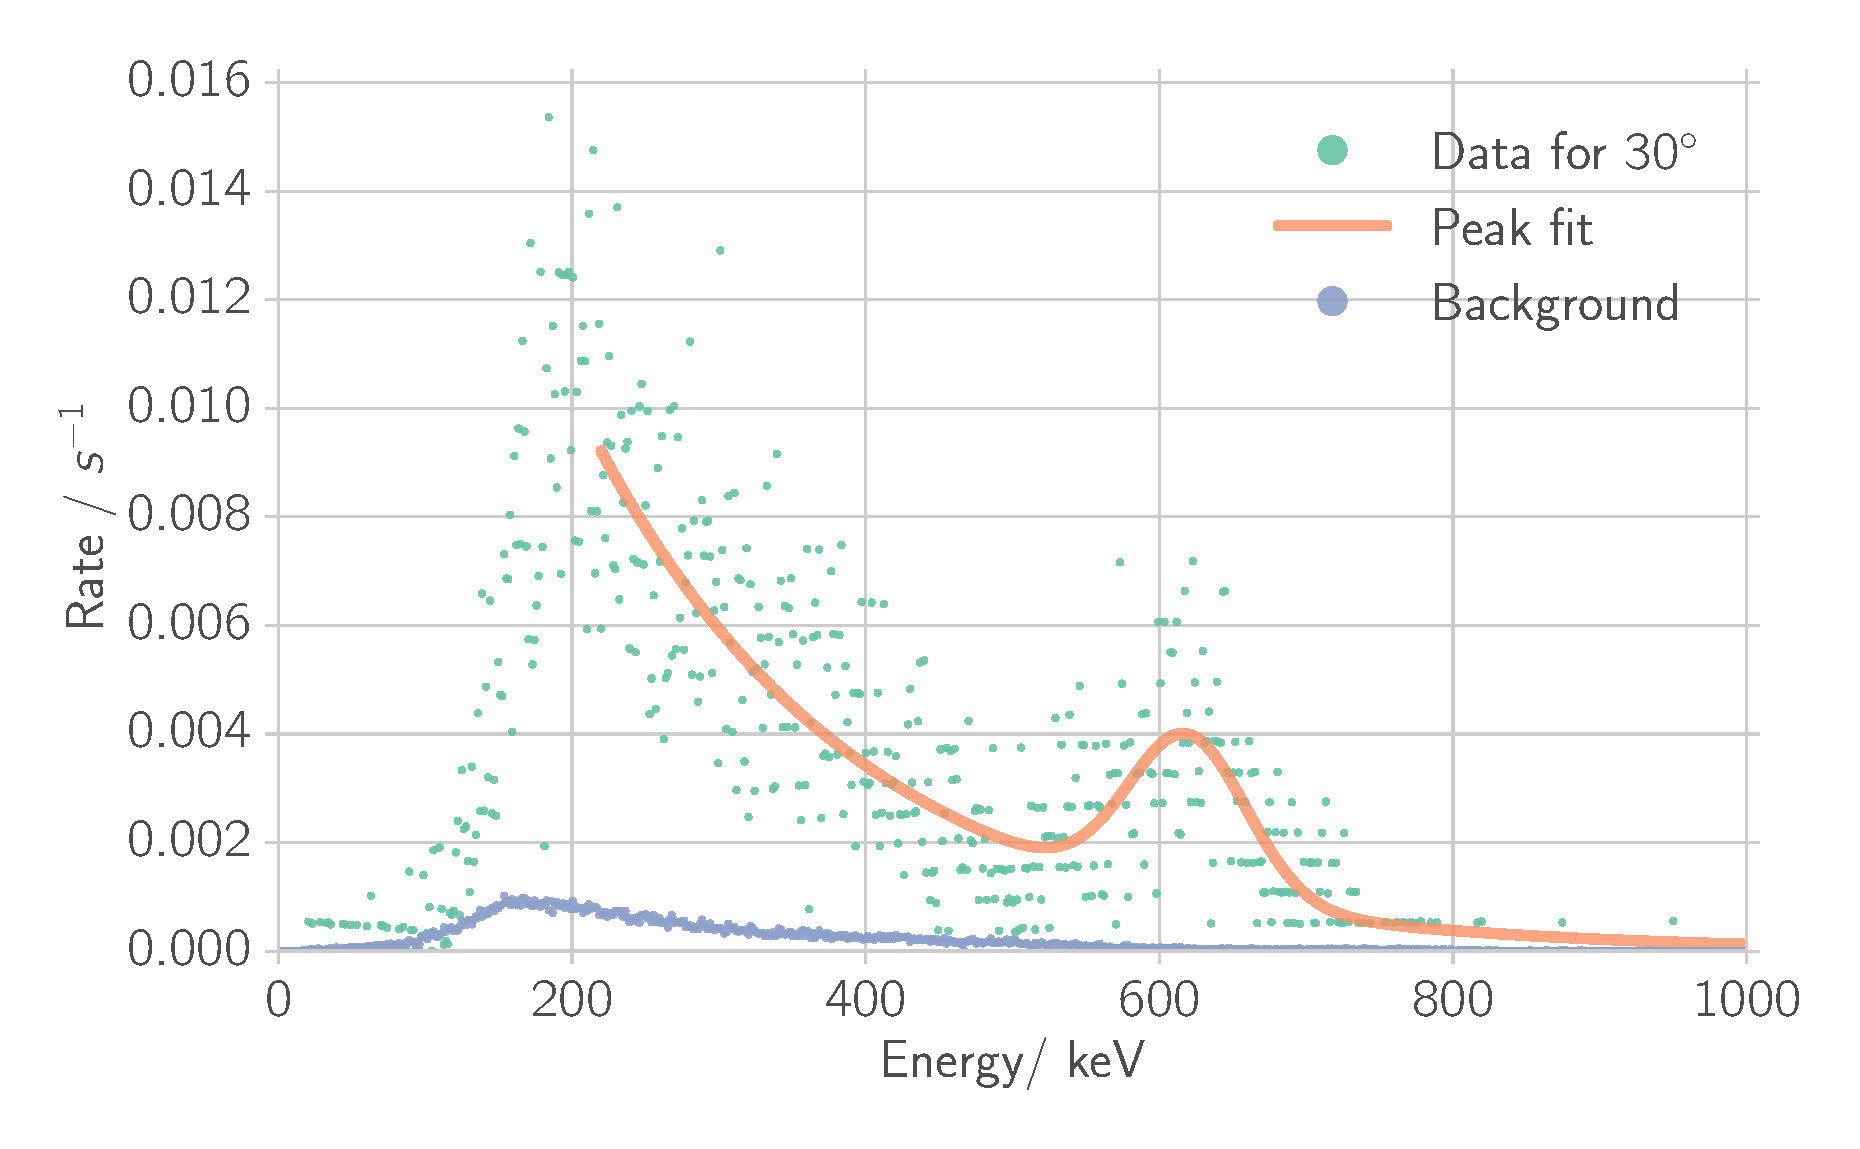
\includegraphics[width=0.9\linewidth]{./analysis/figures/coin_na_30}
    \caption{\textbf{Energy of photons:} Rate of coincident events of 
        NaI scintillator at angle of $\theta = 30^\circ$. The photo peak was approximated
    with a Gaussian distribution. The fit is a scaled Gaussian distribution plus an exponential $c \exp(-b E)$, which
    exhibits the noisy peak from 200 up to 600 keV.}
\label{fig:coin_na_30}
\end{figure}




\begin{figure}[htpb]
    \centering
    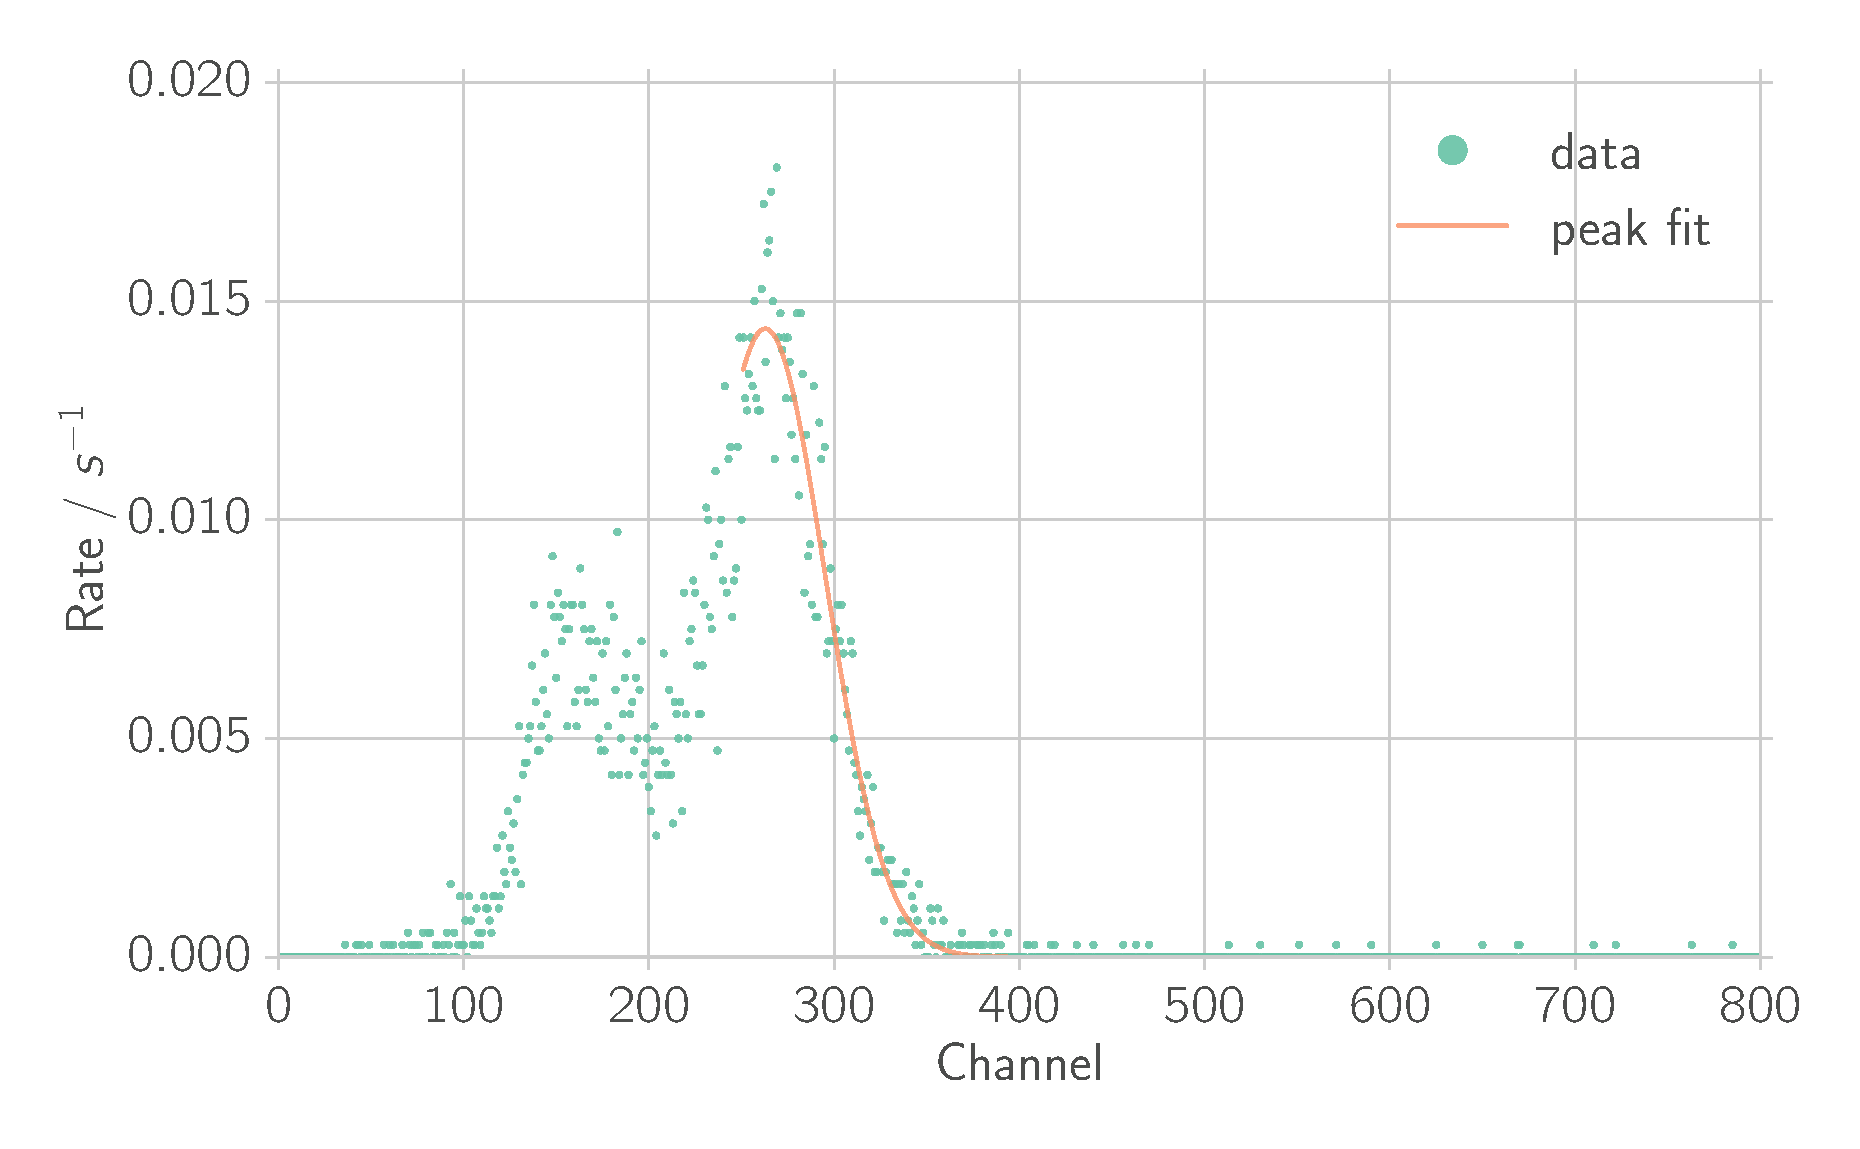
\includegraphics[width=0.9\linewidth]{./analysis/figures/coin_na_90}
\caption{\textbf{Energy of photons:} Rate of coincident events of 
        NaI scintillator at angle of $\theta = 90^\circ$. The distribution 
    was approximated with a Gaussian distribution plus exponential, see figure~\ref{fig:coin_na_30}. }
\label{fig:coin_na_90}
\end{figure}


\begin{figure}[htpb]
    \centering
    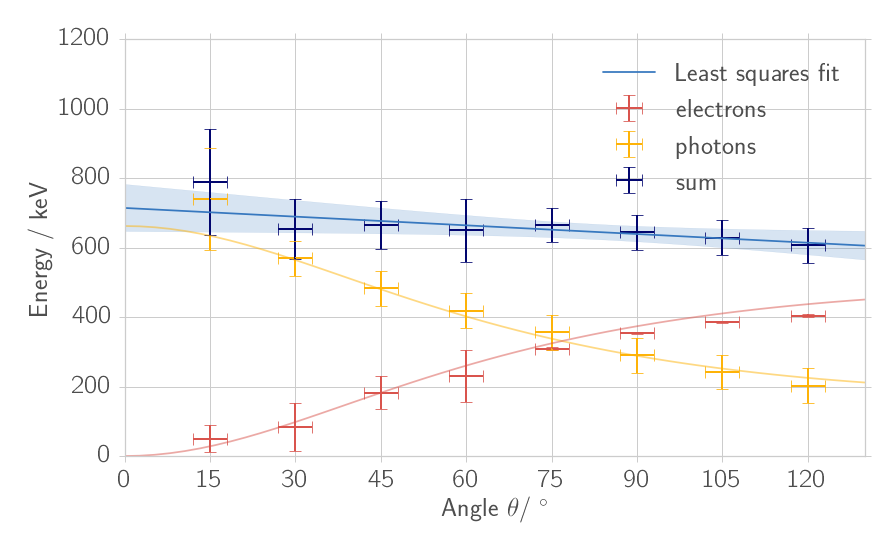
\includegraphics[width=0.9\linewidth]{./analysis/figures/energy_conservation}
    \caption{Summary of the analysis of the foregoing chapter. We arrive at a small tendency of a negative slope, which
    would disagree with energy conservation. However, this tendency is small, it is
    $[-1.1 \pm 0.3]$ keV/$^\circ$ where the height is $[750 \pm 20]$keV.}
\label{fig:energy_conservation}
\end{figure}
\clearpage
\subsection{Differential cross section}
\label{sub:cross_section}
This last section addresses the differential cross section elaborated in section~\ref{sec:cross_section}, which can
be seen as the rate of a photon being detected under an angle of $\theta$. 
For the calculations
we use the fits of the last section, yielding the intensity $I(\theta)$ of coincident photons. Those are compared to the total
intensity $I_\mathrm{total}$ of photons measured in a separate setup. Furthermore we have to take into account the density of
electrons in the material, which is in our case $n_e= 3.4\cdot10^{23}\mathrm{cm}^{-3}$, and the width $d = [1.4 \pm 0.1]$cm. 
Since the PVC scintillator is turned by $\theta / 2$ for a measurement angle $\theta$, we correct for the larger width experienced 
by photons by multiplying with $1 / \cos(\theta / 2)$. 
The cross section (unit in barn, i.e. 1 barn = $10^{24}\mathrm{cm}^{2}$) then reads
\begin{equation}
    \label{eq:cross}
    \frac{\mathrm{d}\sigma}{\mathrm{d} \Omega} = \frac{I_\mathrm{total}}{I(\theta) n_e \cdot d \cdot \delta \omega}
\end{equation}
where we already have implied the dependence on the solid angle $\Delta \Omega$. The solid angle can be seen as the size of the
detector in radial units, which can be calculated via the radius of the NaI scintillator $u=[4.8\pm0.1]$cm and the Distance
between NaI opening and PVC scintillator $U=[11.5\pm0.5]$cm
\begin{equation}
    \Delta \Omega = \frac{\pi u^2}{U^2}  = [0.17 \pm 0.02] \pi.
\end{equation}
Up to now we did not talk about microscopical constraints of the detector, but now we have to consider both the absorption
of the material $\sim \exp(-\mu \cdot d)$ and the efficiency of detection $\epsilon$. Both of this quantities are dependent on the
energy the detector is operating. Correcting equation \eqref{eq:cross} we arrive at
\begin{equation}
\label{eq:diff_cross}
    \frac{\mathrm{d} \sigma}{\mathrm{d} \Omega} = \frac{I_\mathrm{total}}{I(\theta) n_e \cdot d \cdot \delta \omega} \
    \frac{\epsilon(E(\theta = 0 ))}{\epsilon(E(\theta))} \left[ e^{-\mu(E_{\mathrm{total} }) d/2}
    \left( 1 - e^{-\mu(E_{\mathrm{total} }) d/2}  \right)\right]^{-1}.
\end{equation}
The last equation can be understood as follows: We approximate the photon to travel half of the PVC width $d$ with its
primary energy, therefore we need the probability of not being absorbed (hence the factor 1 - exp, if the absorption happen 
in this regime, the scattering will not occur). The other probability accounts for being absorbed in the other half of the width,
leading to an scattering which we can detect. However, this correction is very small and does not change the overall asymptotic
of the curve. The result for our intensities is shown in figure~\ref{fig:na_cross_section}. It is clear that the result is only
correct with respect to the order of magnitude; the dependency with respect to the angle $\theta$ is not fulfilled at all, 
compared to the theoretical prediction of the Klein-Nishina formula calculated before. 

\begin{SCtable}[1.5][tbd]

\caption{Summary of values used for the calculation of the differential cross
  section. Efficiency $\epsilon$ taken from \cite{fluegge} and absorption coefficients $\mu$
  taken from \cite{ver}. The equation for the differential cross section~\eqref{eq:diff_cross} shows that only the 
  coefficient $\epsilon(E(\theta = 0) ) / \epsilon(E(\theta))$ is important for the behavior, for $\mu$ it is slightly
different. }
  \begin{tabular}{lll}
      \rowcolor{LightCyan}  $\theta$ / $^\circ$ & $\mu$ / $\mathrm{cm}^{-1}$ & $\epsilon$ \\ 
      \cellcolor{LightCyan}  0 &    0.089 & 0.40 \\ 
 \cellcolor{LightCyan}  15 &   0.091 & 0.41  \\
 \cellcolor{LightCyan}  30 &   0.091 & 0.45  \\
 \cellcolor{LightCyan}  45 &   0.098 & 0.51  \\
 \cellcolor{LightCyan}  60 &   0.108 & 0.55  \\
 \cellcolor{LightCyan}  75 &   0.120 & 0.63  \\
 \cellcolor{LightCyan}  90 &   0.120 & 0.65  \\
 \cellcolor{LightCyan}  105 &  0.120 & 0.70  \\
 \cellcolor{LightCyan}  120 &  0.136 & 0.80  
  \end{tabular}
    \label{tab:cross}
\end{SCtable}


\begin{figure}[htpb]
    \centering
    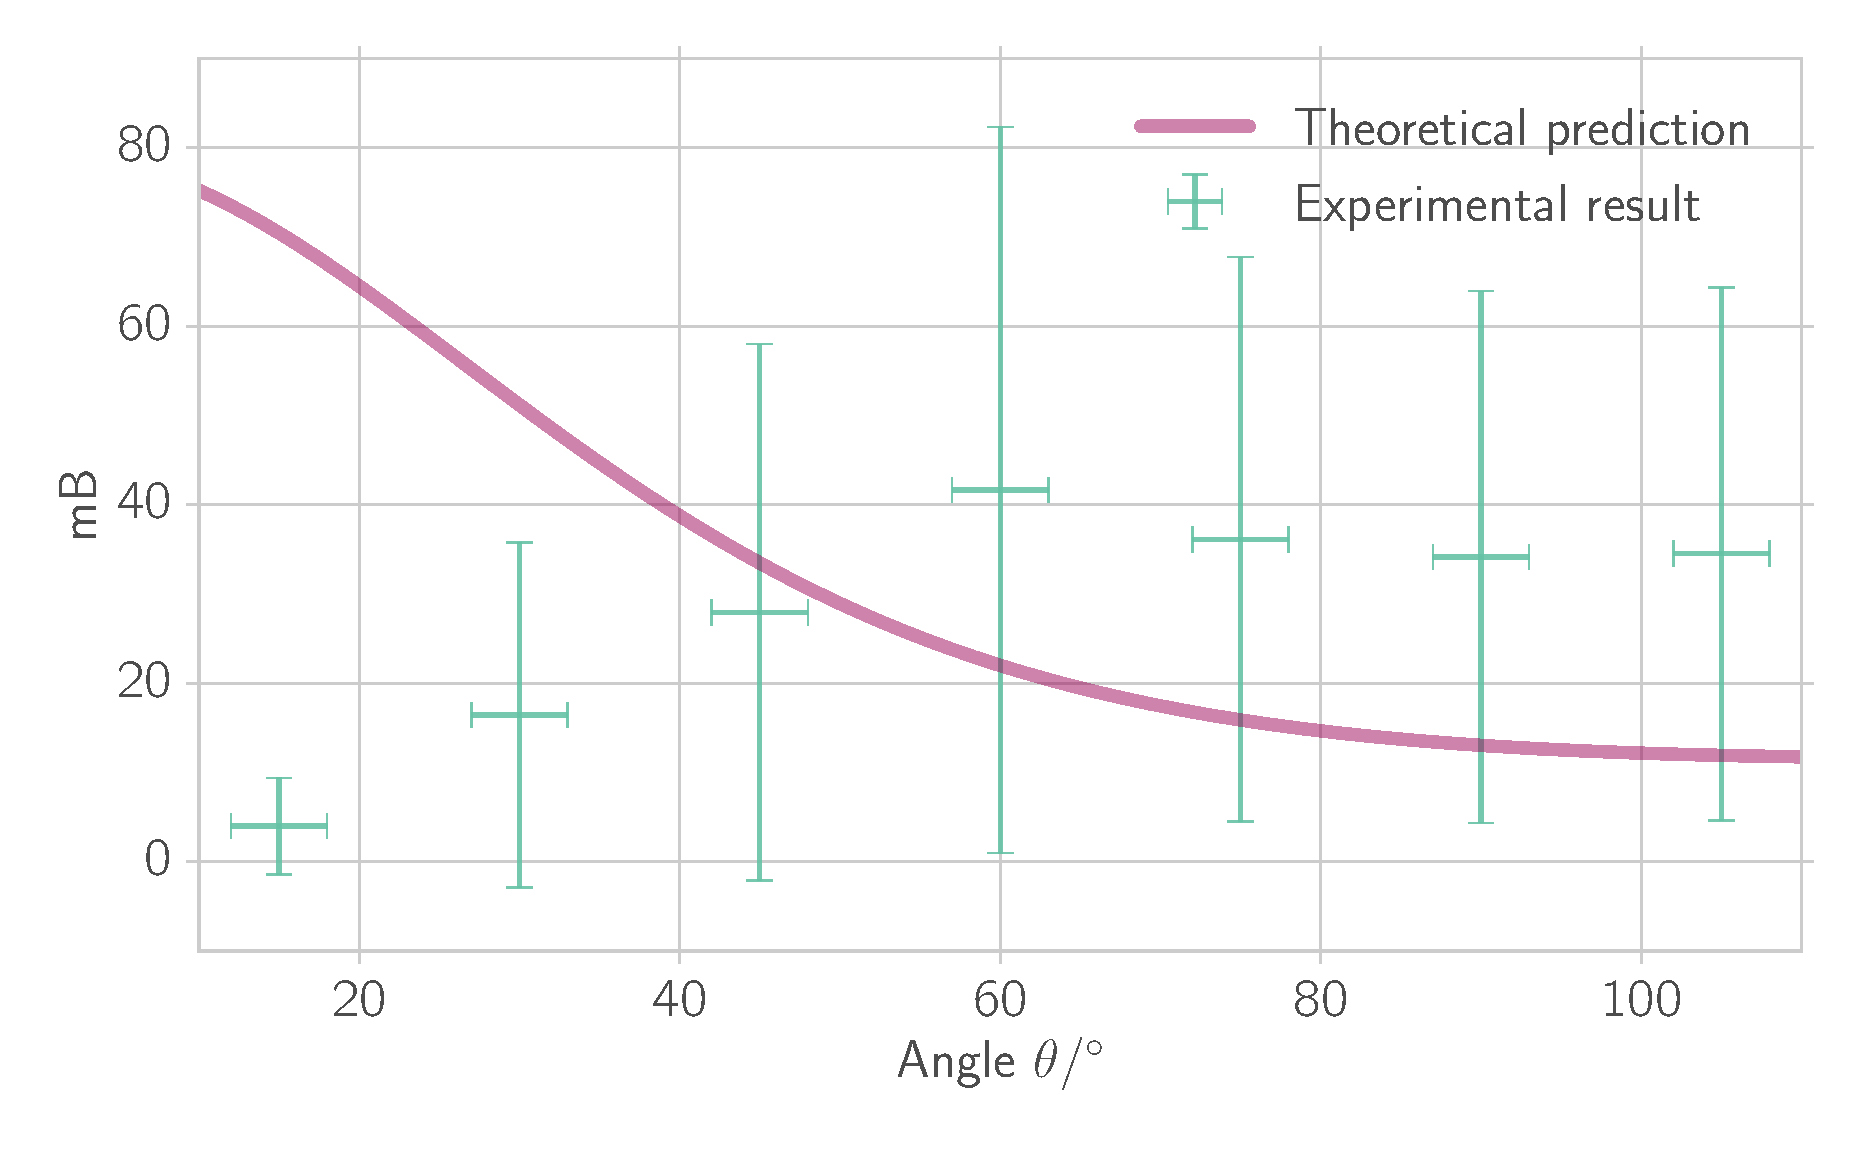
\includegraphics[width=0.9\linewidth]{./analysis/figures/na_cross_section}
    \caption{Experimental results of the differential cross section compared with the theoretical expectation 
        (equation~\eqref{eq:diff_cross}). The experimental data are derived from numerical integration of the measured spectra corrected
        by various intensity or angle dependent. Although good agreement between experiment and theory agree within statistical errors is
        observed, the data is too fraught of errors in order to test for deviations from the theory.}
\label{fig:na_cross_section}
\end{figure}
\newpage
